\documentclass[border=10pt]{standalone}

\usepackage{tikz}
\usepackage{tikzsymbols}
\usetikzlibrary{calc,patterns,shapes.geometric}

\def\centerarc[#1](#2)(#3:#4:#5){\draw[#1] ($(#2)+({#5*cos(#3)},{#5*sin(#3)})$) arc (#3:#4:#5);}

\begin{document}
	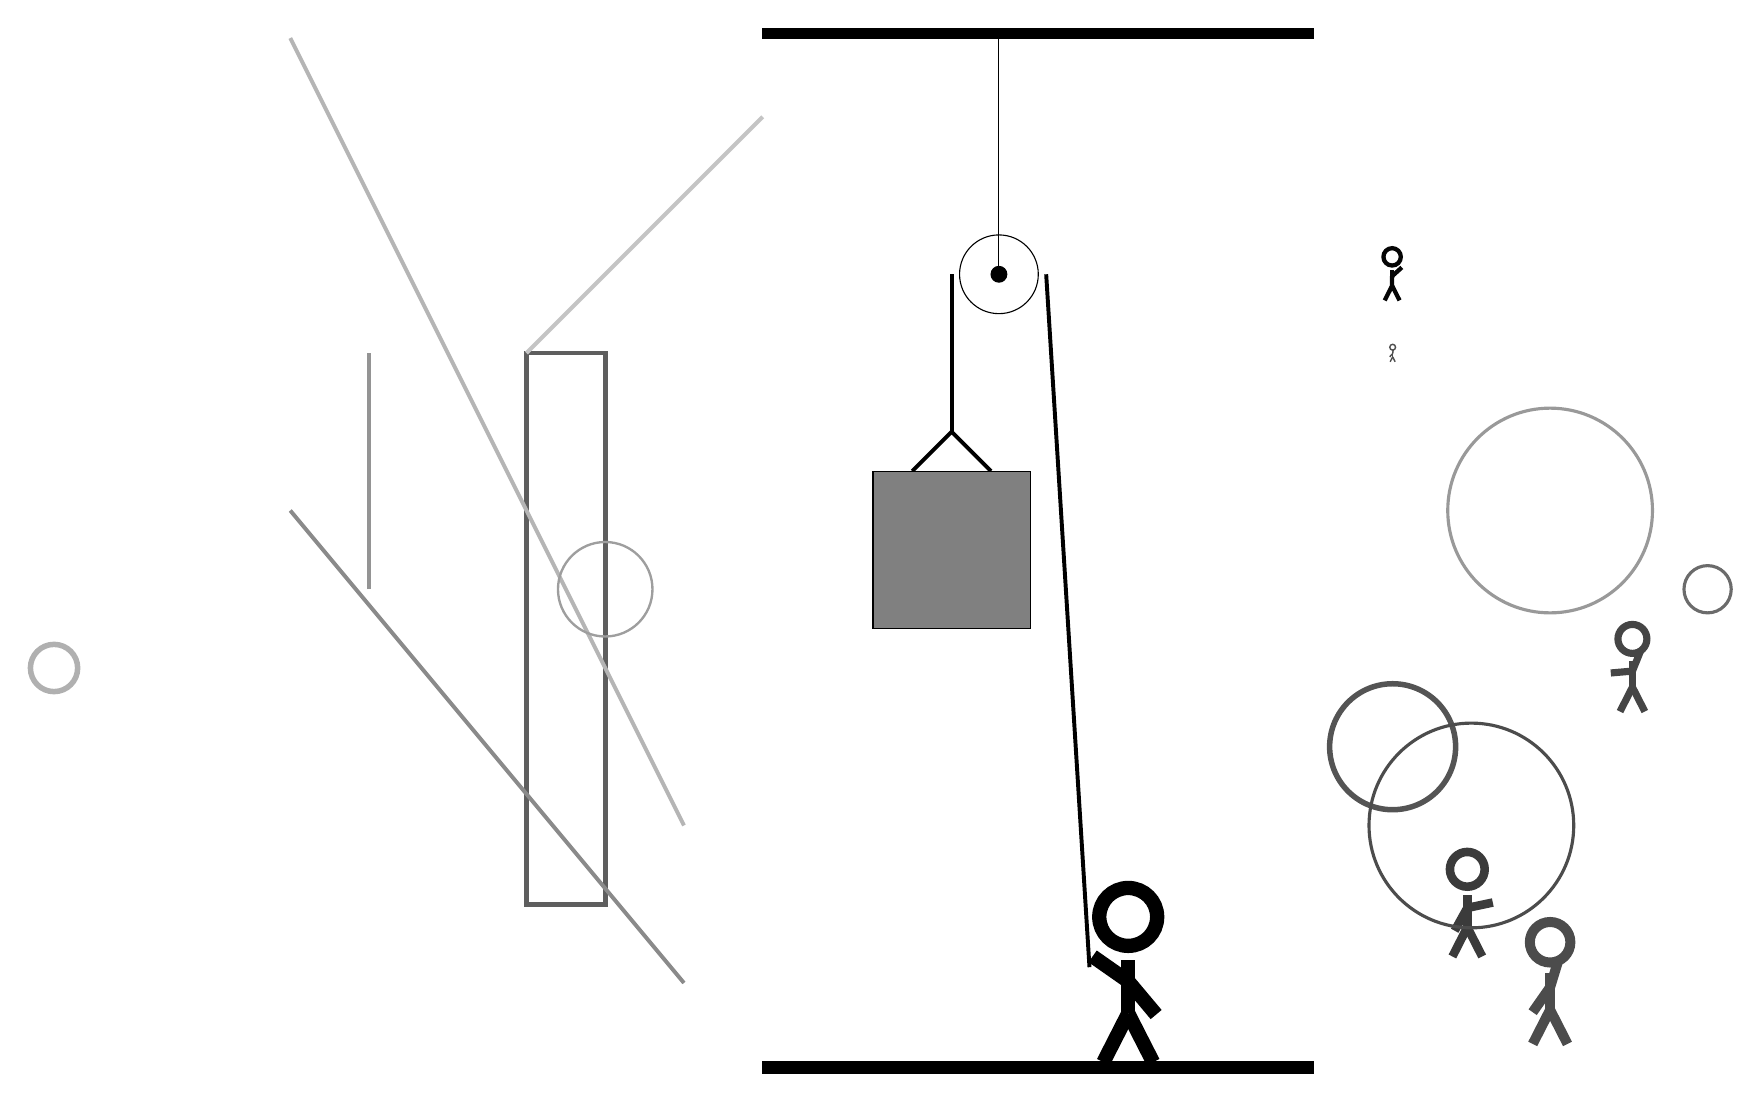
\begin{tikzpicture}
		%%%%% START %%%%%
		
		\draw[fill=black] (-2, 10) rectangle (5, 10.125);
		
		\draw (1, 7) circle (0.5);
		\draw[fill=black] (1, 7) circle (0.1);
		\draw (1, 10) -- (1, 7);
		
		\draw[line width=0.5mm] (-0.1, 4.5) -- (0.4, 5.0) -- (0.9, 4.5);
		\draw[fill=black!50] (-0.6, 4.5) rectangle (1.4, 2.5);
		
		\draw[line width=0.5mm] (0.4, 7) -- (0.4, 5.0);
		\centerarc[line width=0.5mm](1, 7)(0:180:0.6);
		\draw[line width=0.5mm](1.6, 7) -- (2.15, -1.8);
		
		\node at (2.6, -1.9) {\Strichmaxerl[10][-35][-50]};
		
		\draw[line width=0.6mm, color=black!63] (-4, 6) rectangle (-5, -1);
		
		\draw[line width=0.5mm, color=black!46](-3, -2) -- (-8, 4);
		\draw [line width=0.4mm, color=black!58](10, 3) circle (0.3);
		\node[line width=0.2mm, color=black!98] at (6, 7) {\Strichmaxerl[3][89][42]};
		\draw[line width=0.5mm, color=black!29](-3, 0) -- (-8, 10);
		
		\draw[line width=0.5mm, color=black!23](-2, 9) -- (-5, 6);
		\draw [line width=0.7mm, color=black!67](6, 1) circle (0.8);
		
		\draw [line width=0.4mm, color=black!40](8, 4) circle (1.3);
		\draw [line width=0.7mm, color=black!31](-11, 2) circle (0.3);
		
		\node[line width=0.3mm, color=black!77] at (7, -1) {\Strichmaxerl[6][61][12]};
		\node[line width=0.3mm, color=black!69] at (6, 6) {\Strichmaxerl[1][47][82]};
		\draw [line width=0.3mm, color=black!38](-4, 3) circle (0.6);
		\node[line width=0.2mm, color=black!70] at (8, -2) {\Strichmaxerl[7][55][73]};
		\draw[line width=0.5mm, color=black!42](-7, 3) -- (-7, 6);
		\node[line width=0.7mm, color=black!73] at (9, 2) {\Strichmaxerl[5][5][68]};
		\draw [line width=0.4mm, color=black!70](7, 0) circle (1.3);
		
		\draw[fill=black] (-2, -3) rectangle (5, -3.15);
		
		%%%%% END %%%%%
	\end{tikzpicture}
\end{document}